Quando uma substância no estado líquido é confinada em um recipiente, o gás e o líquido atingem o equilíbrio entre si. Sob condições específicas de pressão e temperatura (função da espécie química sob análise), as propriedades físico-químicas de ambas fases convergem para um mesmo ponto até ficarem idênticas. Este ponto é denominado de ponto crítico onde se encerra a interface gás/líquido. Assim, se encontra uma única fase de fluido supercrítico para toda substância que se encontra em condições de pressão e temperatura superiores aos seus parâmetros críticos (temperatura crítica, $T_c$ e pressão crítica, $p_C$. Essa região é melhor visualizada no diagrama de fases mostrada na figura a abaixo (Adaptado de CARRILHO et al., Química Nova. v. 24, nº 4, 2001).

\begin{center}
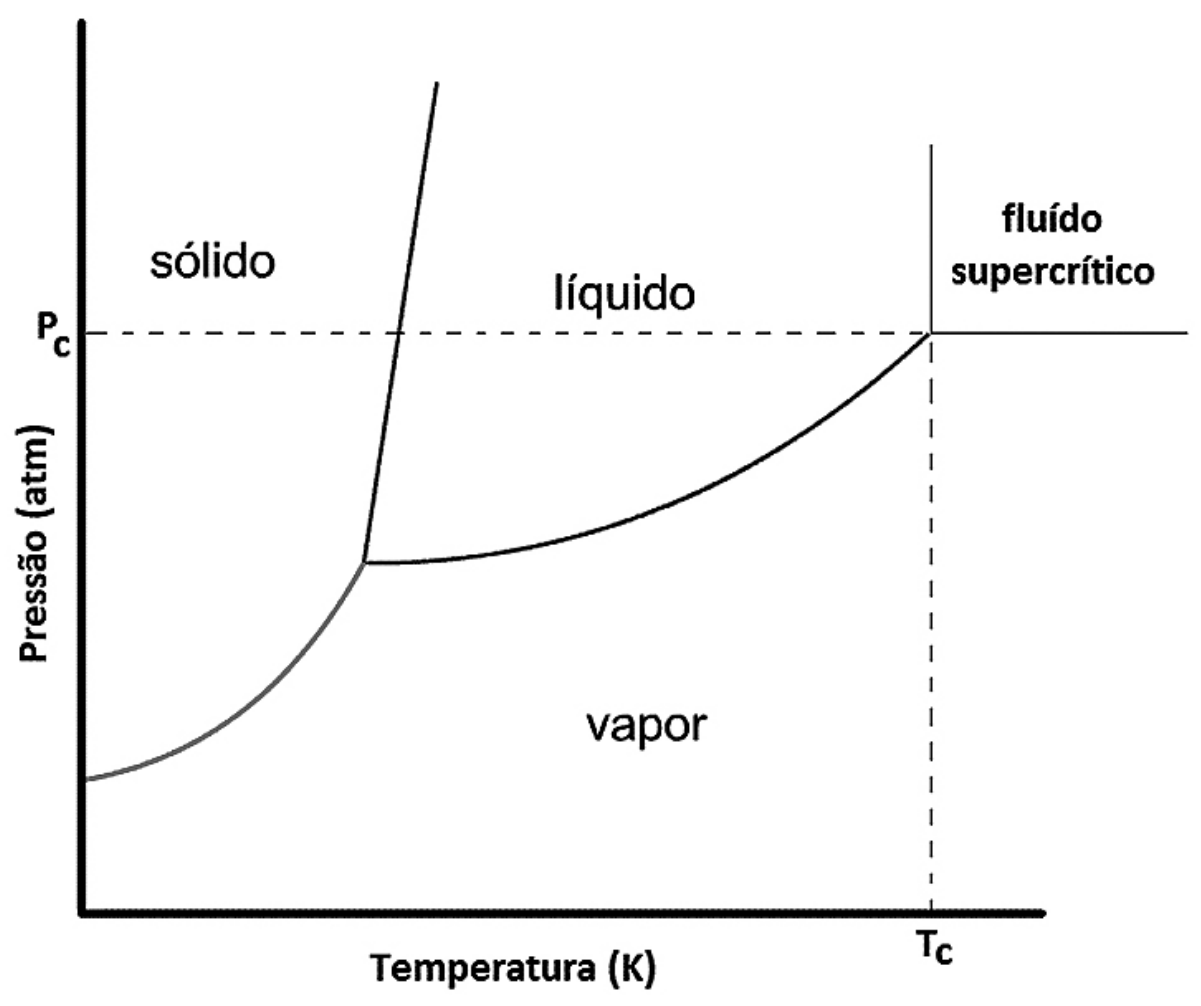
\includegraphics[width=0.35\textwidth]{figure.png}
\end{center}

 Os fluídos supercríticos são muito utilizados para a separação de substâncias, por exemplo, na extração de cafeína para obtenção do café descafeinado. Dentre as substâncias apresentadas abaixo, assinale a alternativa que indica a que possui a menor temperatura crítica ($T_C$). 

 \begin{enumerate}[label = (\alph*)]
	
	\item \chemfig{CO_2} (dióxido de carbono) 
	\item \chemfig{H_3COH} (metanol). 
	\item \chemfig{H_3C[CH_2]_3CH_3} (pentano) 
	\item \chemfig{SF_6} (hexafluoreto de enxofre) 
	\item \chemfig{H_3CCOCH_3} (propanona)
\end{enumerate}
